\documentclass{beamer}
\mode<presentation>
\usepackage{amsmath,amssymb,mathtools}
\usepackage{textcomp}
\usepackage{gensymb}
\usepackage{adjustbox}
\usepackage{subcaption}
\usepackage{enumitem}
\usepackage{multicol}
\usepackage{listings}
\usepackage{url}
\usepackage{graphicx} % <-- needed for images
\def\UrlBreaks{\do\/\do-}

\usetheme{Boadilla}
\usecolortheme{lily}
\setbeamertemplate{footline}{
  \leavevmode%
  \hbox{%
  \begin{beamercolorbox}[wd=\paperwidth,ht=2ex,dp=1ex,right]{author in head/foot}%
    \insertframenumber{} / \inserttotalframenumber\hspace*{2ex}
  \end{beamercolorbox}}%
  \vskip0pt%
}
\setbeamertemplate{navigation symbols}{}

\lstset{
  frame=single,
  breaklines=true,
  columns=fullflexible,
  basicstyle=\ttfamily\tiny   % tiny font so code fits
}

\numberwithin{equation}{section}

% ---- your macros ----
\providecommand{\nCr}[2]{\,^{#1}C_{#2}}
\providecommand{\nPr}[2]{\,^{#1}P_{#2}}
\providecommand{\mbf}{\mathbf}
\providecommand{\pr}[1]{\ensuremath{\Pr\left(#1\right)}}
\providecommand{\qfunc}[1]{\ensuremath{Q\left(#1\right)}}
\providecommand{\sbrak}[1]{\ensuremath{{}\left[#1\right]}}
\providecommand{\lsbrak}[1]{\ensuremath{{}\left[#1\right.}}
\providecommand{\rsbrak}[1]{\ensuremath{\left.#1\right]}}
\providecommand{\brak}[1]{\ensuremath{\left(#1\right)}}
\providecommand{\lbrak}[1]{\ensuremath{\left(#1\right.}}
\providecommand{\rbrak}[1]{\ensuremath{\left.#1\right)}}
\providecommand{\cbrak}[1]{\ensuremath{\left\{#1\right\}}}
\providecommand{\lcbrak}[1]{\ensuremath{\left\{#1\right.}}
\providecommand{\rcbrak}[1]{\ensuremath{\left.#1\right\}}}
\theoremstyle{remark}
\newtheorem{rem}{Remark}
\newcommand{\sgn}{\mathop{\mathrm{sgn}}}
\providecommand{\abs}[1]{\left\vert#1\right\vert}
\providecommand{\res}[1]{\Res\displaylimits_{#1}}
\providecommand{\norm}[1]{\lVert#1\rVert}
\providecommand{\mtx}[1]{\mathbf{#1}}
\providecommand{\mean}[1]{E\left[ #1 \right]}
\providecommand{\fourier}{\overset{\mathcal{F}}{ \rightleftharpoons}}
\providecommand{\system}{\overset{\mathcal{H}}{ \longleftrightarrow}}
\providecommand{\dec}[2]{\ensuremath{\overset{#1}{\underset{#2}{\gtrless}}}}
\newcommand{\myvec}[1]{\ensuremath{\begin{pmatrix}#1\end{pmatrix}}}
\let\vec\mathbf

\title{Matgeo Presentation - Problem 10.7.111}
\author{ee25btech11063 - Vejith}

\begin{document}


\frame{\titlepage}
\begin{frame}{Question}
$\Vec{a}$,$\Vec{b}$,$\Vec{c}$ are three orthogonal vectors. Given that $\vec{a}$=$\hat{i} + 2\hat{j} + 5\hat{k}$ and $\Vec{b}$=$\hat{i} + 2\hat{j} -\hat{k}$, the vector $\vec{c}$ is parallel to \hspace{2.5cm} \brak{\text{IN } 2019}
\begin{enumerate}[label=(\alph*)]
    \begin{multicols}{4}
        \item $\hat{i} + 2\hat{j} + 3\hat{k}$
        \item $2\hat{i} + \hat{j}$
        \item $2\hat{i} - \hat{j}$
        \item $4\hat{k}$
    \end{multicols}
\end{enumerate}
\end{frame}

\begin{frame}{Solution}
Given 
\begin{align}
    \vec{a}=\myvec{1\\2\\5}\\
    \vec{b}=\myvec{1\\2\\-1}\\
    \vec{a}^\top\vec{c}=0\\
    \vec{b}^\top\vec{c}=0
\end{align}
(0.3) and (0.4) can be written as
\begin{align}
    \myvec{\vec{a}^\top \\ \vec{b}^\top}\vec{c}=\myvec{0\\0}\\
    \implies \begin{pmatrix}
        1 & 2 & 5\\
        1 & 2 & -1
    \end{pmatrix}\vec{c}=\myvec{0\\0}
\end{align}
\end{frame}

\begin{frame}{Solution}
Forming the augmented matrix
\begin{align}
    \left(\begin{array}{ccc|c}
        1 & 2 & 5 & 0 \\
        1 & 2 & -1 & 0 
\end{array}\right) &\xleftrightarrow{R_2 \rightarrow R_2- R_1} \left(\begin{array}{ccc|c}
        1 & 2 & 5 & 0 \\
        0 & 0 & -6 & 0 
\end{array}\right)
\end{align}
$\implies$ vector $\vec{c}$ can be written in general as $\vec{c}=\myvec{2k\\-k\\0}$ \brak{\text{for some scalar }k}\\
$\implies$ vector $\vec{c}$ is parallel to $2\hat{i} - \hat{j}$
    \end{frame}

    \begin{frame}{Plot}
        \begin{figure}
            \centering
            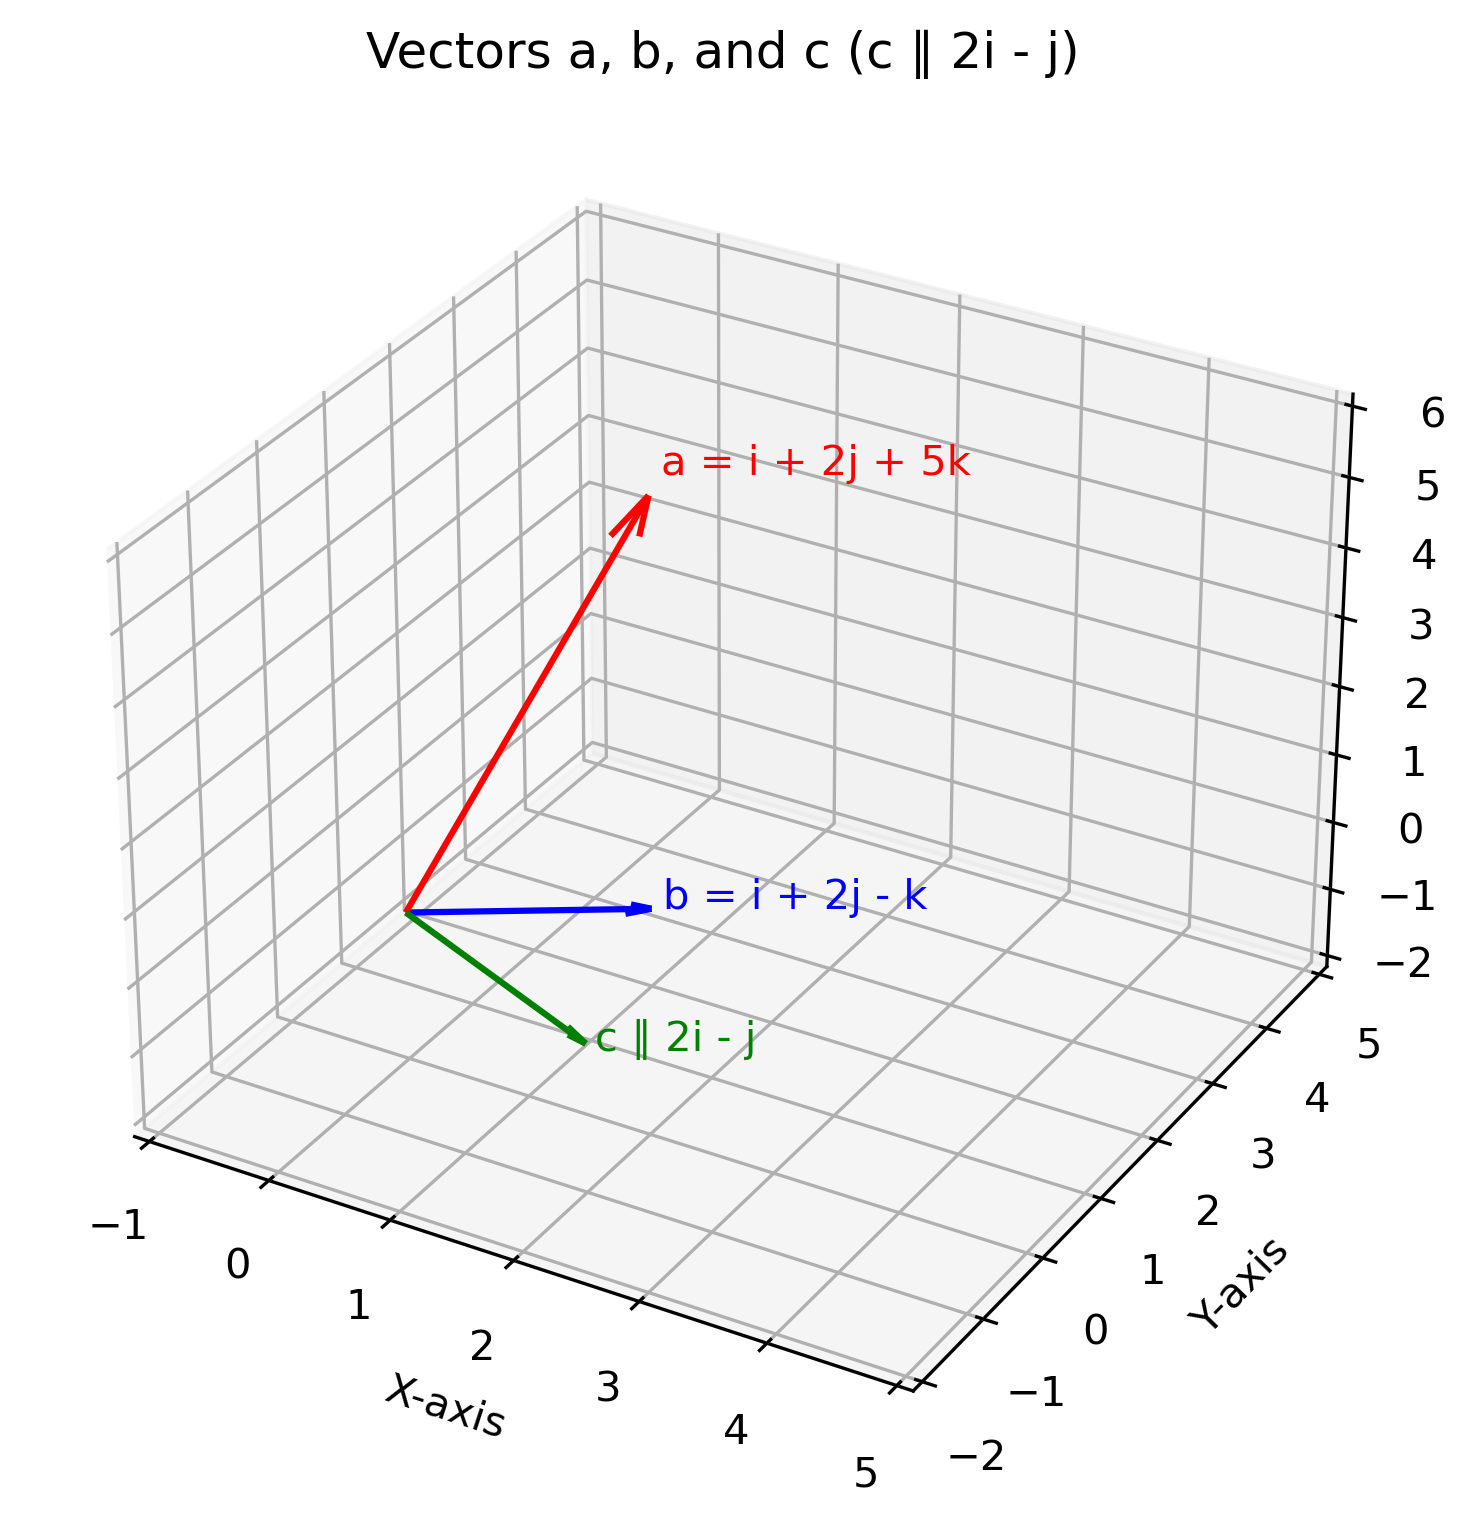
\includegraphics[width=0.65\columnwidth]{figs/01.png}
            \caption{Caption}
            \label{fig:placeholder}
        \end{figure}
    \end{frame}

    % --------- CODE APPENDIX ---------
\section*{Appendix: Code}

% C program
\begin{frame}[fragile]{C Code: vector.c}
\begin{lstlisting}[language=C]
#include <stdio.h>

int main() {
    // Given vectors
    float a[3] = {1, 2, 5};
    float b[3] = {1, 2, -1};

    // Variables for the unknown vector c = (x, y, z)
    // We will solve the system:
    // a·c = 0  =>  x + 2y + 5z = 0
    // b·c = 0  =>  x + 2y - z = 0

    float A[2][3] = {
        {1, 2, 5},
        {1, 2, -1}
    };
    float x, y, z;

    // Using elimination (matrix method):
    // Subtract equation 2 from equation 1
    // (1 - 1)x + (2 - 2)y + (5 - (-1))z = 0 - 0
    // => 6z = 0 => z = 0

    z = 0;

    // Substitute z = 0 in first equation:
    // x + 2y + 5*0 = 0 => x = -2y
    // Let y = 1 (for direction vector)

    y = 1;
    x = -2 * y;
\end{lstlisting}
\end{frame}

\begin{frame}[fragile]{C Code: vector.c}
\begin{lstlisting}[language=C]
    // Vector c is proportional to (-2, 1, 0)
    // Parallel vector can be written as (2, -1, 0)

    FILE *fp;
    fp = fopen("vector.dat", "w");

    if (fp == NULL) {
        printf("Error opening file!\n");
        return 1;
    }

    fprintf(fp, "Vector c is parallel to: 2i - j\n");
    fprintf(fp, "Hence, c is parallel to (2, -1, 0)\n");

    fclose(fp);

    printf("Result written to vector.dat successfully.\n");

    return 0;
}


\end{lstlisting}
\end{frame}

% Python plotting
\begin{frame}[fragile]{Python: plot.py}
\begin{lstlisting}[language=Python]
import numpy as np
import matplotlib.pyplot as plt
from mpl_toolkits.mplot3d import Axes3D

# Given vectors
a = np.array([1, 2, 5])
b = np.array([1, 2, -1])

# Vector c is parallel to 2i - j
c = np.array([2, -1, 0])

# Verify orthogonality (dot products)
dot_a_c = np.dot(a, c)
dot_b_c = np.dot(b, c)

print("a · c =", dot_a_c)
print("b · c =", dot_b_c)
print("\nSince both dot products are 0, c is orthogonal to both a and b.")
print("Hence, c is parallel to 2i - j.\n")

# Plot setup
fig = plt.figure(figsize=(8, 6))
ax = fig.add_subplot(111, projection='3d')

# Plot vectors
ax.quiver(0, 0, 0, a[0], a[1], a[2], color='r', arrow_length_ratio=0.1)
ax.quiver(0, 0, 0, b[0], b[1], b[2], color='b', arrow_length_ratio=0.1)
ax.quiver(0, 0, 0, c[0], c[1], c[2], color='g', arrow_length_ratio=0.1)

# Label each vector beside its arrow
ax.text(a[0]*1.05, a[1]*1.05, a[2]*1.05, 'a = i + 2j + 5k', color='r', fontsize=10)
\end{lstlisting}
\end{frame}


\begin{frame}[fragile]{Python: plot.py}
\begin{lstlisting}[language=Python]
ax.text(b[0]*1.05, b[1]*1.05, b[2]*1.05, 'b = i + 2j - k', color='b', fontsize=10)
ax.text(c[0]*1.05, c[1]*1.05, c[2]*1.05, 'c ∥ 2i - j', color='g', fontsize=10)

# Axis labels and style
ax.set_xlabel('X-axis')
ax.set_ylabel('Y-axis')
ax.set_zlabel('Z-axis')
ax.set_xlim([-1, 5])
ax.set_ylim([-2, 5])
ax.set_zlim([-2, 6])
ax.set_title('Vectors a, b, and c (c ∥ 2i - j)')
ax.grid(True)

# Save the figure
plt.savefig("vectors_plot.png", dpi=300, bbox_inches='tight')
print("Figure saved as 'vectors_plot.png' successfully.")

# Show the plot
plt.show()

\end{lstlisting}
\end{frame}
\end{document}
